\documentclass[conference]{IEEEtran}
\IEEEoverridecommandlockouts
% The preceding line is only needed to identify funding in the first footnote. If that is unneeded, please comment it out.
\usepackage{cite}
\usepackage{amsmath,amssymb,amsfonts}
\usepackage{algorithmic}
\usepackage{graphicx}
\usepackage{textcomp}
\usepackage{xcolor}
\usepackage{acronym}
\usepackage{listings}
\usepackage{setspace}
\usepackage{url}
\usepackage[utf8]{inputenc}
\def\BibTeX{{\rm B\kern-.05em{\sc i\kern-.025em b}\kern-.08em
    T\kern-.1667em\lower.7ex\hbox{E}\kern-.125emX}}
\begin{document}
	
\newacro{CGRA}{Coarse-Grain Reconfigurable Array}
\newacro{CPU}{Central Processing Unit}
\newacro{ISA}{Instruction Set Architecture}
\newacro{UART}{Universal Asynchronous Receiver-Transmitter}
\newacro{LED}{Light Emitting Diode}
\newacro{CM}{Configuration Module}
\newacro{DE}{Data Engine}
\newacro{FU}{Functional Units}
\newacro{AGU}{Address Generation Unit}
\newacro{LUT}{Lookup Tables}
\newacro{FPGA}{Field-Programmable Gate Array}
\newacro{ASIC}{Application-Specific Integrated Circuit}
\newacro{CPI}{Cycles Per Instruction}
\newacro{CNN}{Convolutional Neural Network}
\newacro{HDL}{Hardware Description Language}
\newacro{RTL}{Register-Transfer Level}
\newacro{UUT}{Unit Under Test}
\newacro{VPI}{Verilog Procedural Interface}
\newacro{API}{Application Programming Interface}
\newacro{DMA}{Direct Memory Access}
\newacro{VCD}{Value Change Dump}
\newacro{BRAM}{Block Random Access Memories}
\newacro{DSP}{Digital Signal Processor}
\newacro{ASIP}{Application Specific Instruction Set Processors}
\newacro{ALU}{Arithmetic Logic Unit}


\title{Simulator for the RV32-Versat architecture\\ }

\author{\IEEEauthorblockN{João César Martins Moutoso Ratinho}
\IEEEauthorblockA{\textit{Electrical and Computer Engineering Department} \\
\textit{Instituto Superior Técnico}\\
Lisbon, Portugal \\
joao.ratinho@tecnico.ulisboa.pt}
}

\maketitle

\begin{abstract}
This paper presents a new simulation environment for the RV32-Versat system
using the Verilator simulation framework. The RV32-Versat system consists of the
PicoRV32 RISC-V processor connected to the Versat \ac{CGRA} architecture. This new 
simulation environment presents significant advantages over
the typical simulation environments using commercial event-driven
simulators. The first advantage is speed: the new environment is considerably
faster, therefore saving valuable time when developing applications for the
RV32-Versat architecture. The second advantage is cost: Verilator is available
under a free open-source licence, while the typical event-driven simulators
require very expensive licences, hard to justify for small companies and
projects. The third and last advantage is the easy support for hardware and
software co-simulation. The event-driven simulators are lacking in this field,
but the new environment using Verilator solves this problem, allowing a seamless
integration through C++ or SystemC. This new simulation environment is the
result of a detailed study of the state of the art of \ac{CPU} and \ac{CGRA}
simulation and the RV32-Versat architecture, also presented in this paper.
\end{abstract}

\begin{IEEEkeywords}
Coarse-Grain Reconfigurable Arrays, Simulation Environment,
Verilator, CGRA Simulation, High-Level Simulation,
Co-Simulation
\end{IEEEkeywords}

%%%%%%%%%%%%%%%%%%%%%%%%%%%%%%%%%%%%%%%%%%%%%%%%%%%%%%%%%%%%%%%%%%%%%%%%%%%%%%%%%%%%%%%%%%

\section{Introduction}
\IEEEPARstart{I}{n} any digital circuit simulation is fundamental to verify if the 
circuit is working properly in the different stages of its development. The motivation for
this paper became clear when I started working with Versat about a year ago, in
the context of an internship in which I had the opportunity to participate in
the development of an MP3 encoder. During that project I was able to understand
the main limitations of the simulation environments using traditional
simulators: they are slow with complex simulations, many times require costly
licences and they provide a difficult integration of software / hardware
co-simulation, many times leading to the use of ad hoc solutions.

These limitations gave me the motivation to look for a solution that would
address them, therefore making the simulation process during a project faster,
cheaper, more efficient and with an integrated support for software and hardware
co-simulation. That way, industrial projects like the one I participated in
could be done in a much more efficient way, which can be very important for
companies with little resources.

Therefore, the main objective of this paper is to develop a new simulation environment 
for the RV32-Versat that is able to overcome the typical problems inherent to the use of
simulation environments based in traditional simulators, as referred before.

Consequently, the new simulation environment has three main objectives. The
first one is being considerably faster than simulating the RV32-Versat
architecture with commercial simulators. This can be particularly useful when
developing new applications for this architecture, since it saves time during
the debug process. The second objective is being cheaper than traditional
simulators, saving resources. Finally, the third objective is to support
hardware and software co-simulation in an integrated environment rather than
using special interfaces and/or ad hoc solutions.

Fulfilling these objectives required studying the current state of the art of
the simulators and the RV32-Versat architecture. This way, it was possible to
understand what types of simulators are more suitable for the Versat
architecture. To validate the simulation environment, a convolutional neural
network application for recognizing hand-written digits was developed.
This application was also used to benchmark different commercially
available simulators.

%%%%%%%%%%%%%%%%%%%%%%%%%%%%%%%%%%%%%%%%%%%%%%%%%%%%%%%%%%%%%%%%%%%%%%%%%%%%%%%%%%%%%%%%%%

\section{The RV32-Versat architecture}
\label{chapter:rv32-versat}

\begin{figure}[!htb]
	\centering
	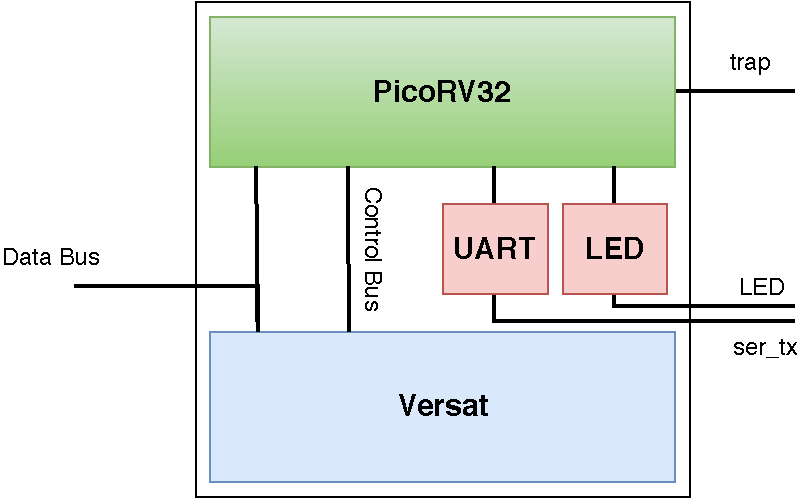
\includegraphics[width=0.4\textwidth]{Figures/rv32-versat.pdf}
	\caption{RV32-Versat top-level diagram.}
	\label{fig:rv32-versat}
\end{figure}

The RV32-Versat architecture was developed during this paper, by a team of 3
people including the author. The starting point was the Versat
\ac{CGRA}~\cite{sousa:versat, sousa:versat2016, sousa:controller,
	sousa:compiler, versat:specification}. A \acf{CGRA} is a collection of programmable 
\ac{FU} and embedded memories connected by programmable interconnects, forming the 
reconfigurable array. For a given set of configuration bits, the reconfigurable
array forms a hardware datapath that can execute an algorithm orders of magnitude faster 
than a conventional \ac{CPU}. This type of architectures can be used as hardware 
co-processors to accelerate algorithms that are time/power consuming in general purpose 
\ac{CPU}s.

This \ac{CGRA} could only be programmed
in assembly language which, despite being great for optimising algorithms, it
was a problem when creating complex and lengthy algorithms. Thus, by removing
its controller (called PicoVersat) and replacing it by the PicoRV32
processor~\cite{cliffordwolf:picorv32}, with a RISC-V \ac{ISA}, this problem was
solved since now Versat can be programmed in the C/C++ language via the PicoRV32
processor. Versat will work as a peripheral of the processor for accelerating
parts of the program, using an interface of C++ classes created for this
purpose, as is explained in Section~\ref{section:programming}.

The RV32-Versat architecture is shown in Figure~\ref{fig:rv32-versat}, and it
comprises two main modules: the PicoRV32 processor and the Versat \ac{CGRA}.
There are also two additional modules in the RV32-Versat: the \ac{UART} and the
\ac{LED}.  Both modules are used for debugging. In this context the \ac{UART}
module is particularly useful, given that it allows to print values in the
computer terminal when simulating or testing the circuit. The LED provides an
even simpler debug mechanism when everything else fails.


As can be seen in the figure, the databus can be used to access the Versat's
memories with values from the PicoRV32 controller, external host or \ac{DMA}
master or, in simulation, by the testbench. This bus is used to upload
Versat with data to be processed and to download data already processed by
Versat. In case a testbench is used, hexadecimal files containing the input and
output data can be used, which is useful for debugging when developing new
applications. The data bus is comprised of the signals data databus\_sel (global
bus select), databus\_rnw (read / not write signal), databus\_addr (address),
databus\_data\_in (input data to PicoRV32) and databus\_data\_out (output data to
PicoRV32).

Other changes were made to Versat in order to adapt it for the RV32-Versat
architecture. One of these changes was the creation of a C++ driver, as detailed
in section~\ref{section:programming}, that allows the user to program Versat
using C++ classes. For that, the user just needs to include the respective {\tt
	versatUI.hpp} header file and link the driver functions. This is a major
improvement, since previously Versat could only be programmed in Assembly,
whereas now it can be programmed using its C++ classes inside of a C or C++ code
that runs in the PicoRV32 processor, which is more user-friendly.

As detailed in Section~\ref{section:picorv32}, the PicoRV32 processor is far
from being a fast processor, since its main purpose is to be a small processor
with low power consumption. However, the impact that this has in the overall
performance of the system is attenuated by the use of Versat to speed up the
time consuming parts of the algorithms implemented in this system. This means
that the RV32-Versat is expected to have a performance similar to processors
with more resources (in terms of area and power consumption).


\subsection{The Versat architecture}
\label{section:versat}

\begin{figure}[!htb]
	\centering
	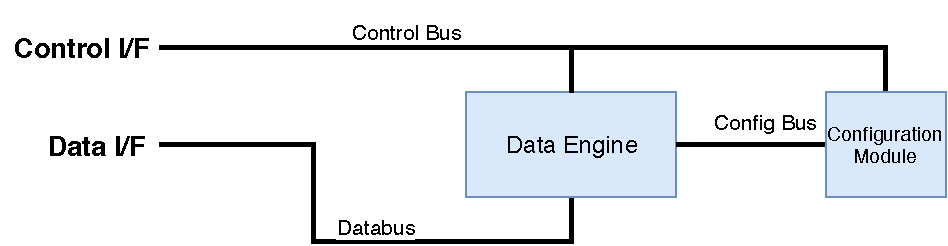
\includegraphics[width=0.4\textwidth]{Figures/top.pdf}
	\caption{Versat top-level entity.}
	\label{fig:top}
\end{figure}

The Versat CGRA architecture~\cite{sousa:versat, sousa:versat2016,
	sousa:controller, sousa:compiler, versat:specification} used in RV32-Versat is
shown in Figure~\ref{fig:top}, and it consists of two main modules: the Data
Engine and the Configuration Module. The Controller, Program Memory and Control
Register File that were previously included in the Versat architecture were
removed for the RV32-Versat system, given that in this new architecture the
Versat works as a peripheral, being controlled by the PicoRV32 processor.

The Versat core has a Control and a Data interface. The Control interface is
used by PicoRV32 processor to instruct Versat to load and execute programs. On
the other hand, the Data interface is used to load and read data from Versat.

Versat user programs can use the \ac{DE} to carry out data intensive computations. To
perform these computations, the PicoRV32 processor writes \ac{DE} configurations to
the \ac{CM}, through the host or memory interface, or simply restores
configurations previously stored in the \ac{CM}. The PicoRV32 can also load the
\ac{DE} with data to be processed or save the processed data back in the
external memory using the Data interface. This interface can also be used to
initially load the Versat program or to move \ac{CGRA} configurations between
the core and the external memory.


%%%%%%%%%%%%%%%%%%%%%%%%%%%%%%%%%%%%%%%%%%%%%%%%%%%%%%%%%%%%%%%%%%%%%%%%
\subsubsection{Data Engine}
\label{subsection:data}

\begin{figure}[!htb]
	\centering
	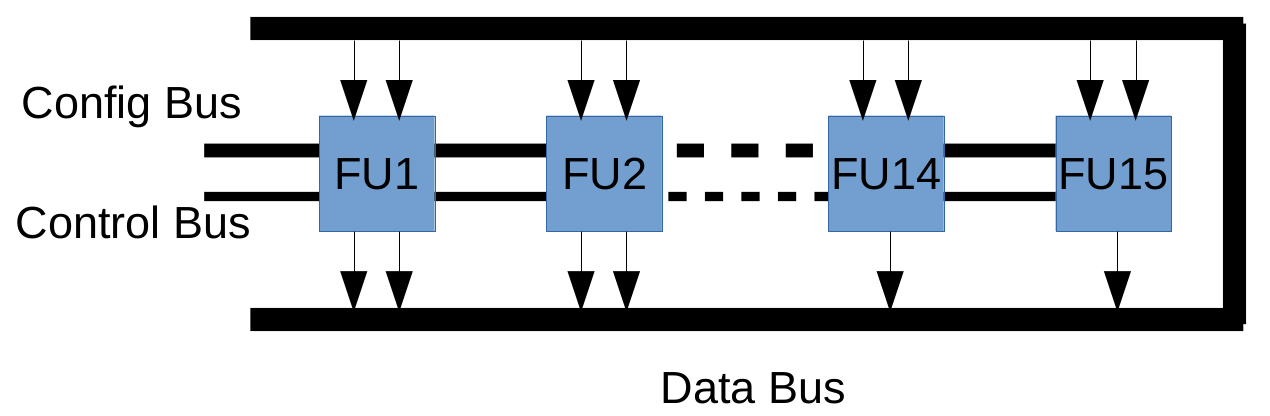
\includegraphics[width=0.4\textwidth]{Figures/de.png}
	\caption{Versat data engine.}
	\label{fig:de}
\end{figure}

The \ac{DE} has a flexible topology, in which the user can configure the number
of \ac{FU} and their respective types. In Figure~\ref{fig:de} it is shown a
\ac{DE} example with 15 \ac{FU}s. The \ac{DE} is a 32-bit architecture with the
following configurable \ac{FU}s: Arithmetic and Logic Unit (ALULite),
Multiplier Accumulator (Muladd), Barrel Shifter (BS) and dual-port 16kB embedded
memories (MEM).

The \ac{FU}s are interconnected by a wide bus called the Data Bus. This bus is
the concatenation of all \ac{FU} outputs, with each FU contributing with a
32-bit section to the Data Bus. An embedded memory contributes 2 sections to the
Data Bus, since it has 2 ports. The Data Bus allows for a maximum of 19
sections, and these sections can be selected by each FU, according to the
configurations that they receive from the respective configuration registers in
the \ac{CM}, whose outputs are concatenated in another wide bus called the
Config Bus.

The \ac{DE} has a full mesh topology, meaning that each FU can select any
\ac{FU} output as one of its inputs. This kind of structure may seem unnecessary
but it greatly simplifies the compiler design as it avoids expensive place and
route algorithms~\cite{sousa:versat2016}. It also facilitates the configuration
of the different datapaths, because the user doesn't need to remember or check
what is connected to what since all the \ac{FU}s are interconnected.

%%%%%%%%%%%%%%%%%%%%%%%%%%%%%%%%%%%%%%%%%%%%%%%%%%%%%%%%%%%%%%%%%%%%%%%%
\subsubsection{Configuration Module}
\label{subsection:configuration}

In Versat, the configuration bits are organized in configuration spaces, one for
each \ac{FU}. Each configuration space comprises multiple fields, which are memory
mapped from the Controller (PicoRV32) point of view. Thus, the Controller is able to
change a single configuration field of an FU by writing to the respective address. This
implements partial reconfiguration.

The \ac{CM} contains a register file with a variable length (the length depends on the 
\ac{FU} used), a shadow register and a memory. The shadow register holds the current
configuration of the \ac{DE}, which is copied from the main configuration register
whenever the Update signal is activated. This means that the configuration
register can be changed in the main register while the \ac{DE} is running.


%%%%%%%%%%%%%%%%%%%%%%%%%%%%%%%%%%%%%%%%%%%%%%%%%%%%%%%%%%%%%%%%%%%%%%%%
\subsection{The PicoRV32 architecture}
\label{section:picorv32}

The \ac{CPU} architecture used in the RV32-Versat system is the PicoRV32
architecture~\cite{cliffordwolf:picorv32}. It implements the RISC-V RV32IMC
instruction set and is publicly available under a free and open hardware
licence. This processor has a small size (750-2000 \ac{LUT} in 7-Series Xilinx
Architecture), and was originally meant to be used as an auxiliary processor in
\ac{FPGA} designs and \ac{ASIC}. Also, its high maximum frequency of operation
(250-450 MHz on 7-Series Xilinx FPGAs) means that it can be integrated in most
existing designs without crossing clock domains.

The average \ac{CPI} is approximately 4, depending on the mix of instructions in the 
code, meaning that the PicoRV32 is far from being a fast processor. However, this was 
already expected, since the main purpose of this processor is to have a small area and 
power consumption. Also, the high maximum clock frequency allowed by this processor 
reduces the performance impact of the high \ac{CPI} values.

%%%%%%%%%%%%%%%%%%%%%%%%%%%%%%%%%%%%%%%%%%%%%%%%%%%%%%%%%%%%%%%%%%%%%%%

\subsection{Programming RV32-Versat}
\label{section:programming}

In order to allow the user to program Versat in an intuitive way using PicoRV32
as a controller, a driver was created. It consists of a C++ header file called
versatUI.hpp, a C++ file file called {\tt versat\_func.cpp} and a python script called
{\tt xdictgen}. The {\tt versatUI.hpp} file, included in the {\tt versat\_func.cpp} file, 
contains multiple C++ classes, one for each type of functional unit, that contain
constructors that allow configuring the different functional units used in
Versat. Each class was implemented with
multiple functions, this way allowing the configuration of only the necessary
parameters (instead of all the parameters), taking advantage of Versat's partial
reconfiguration capabilities.

The {\tt xdictgen} python script was created to read the Versat Verilog include
files, extract the constants, and create a file called {\tt versat\_defs.hpp} with
all these constants. This file will then be included in the {\tt versatUI.hpp} file and
in the C code that runs in the PicoRV32 processor, making the Versat
configuration constants available in these files. This way, when configuring the
different functional units available, the user does not need to remember the
value of the different constants, instead she/he just needs to know their name.

%%%%%%%%%%%%%%%%%%%%%%%%%%%%%%%%%%%%%%%%%%%%%%%%%%%%%%%%%%%%%%%%%%%%%%%%
\subsection{Application Example}
\label{section:application}

\begin{figure}[!htb]
	\centering
	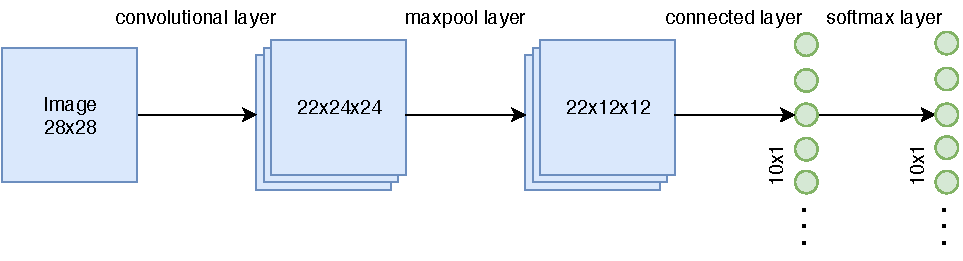
\includegraphics[width=0.4\textwidth]{Figures/CNN_architecture.pdf}
	\caption{CNN architecture implemented in RV32-Versat.}
	\label{fig:cnn}
\end{figure}

To fully test the system and the simulation environment an application using a previously
trained \ac{CNN} for digit classification in different images
was developed for the RV32-Versat. This application was based on a simple \ac{CNN} 
developed by the professor Horácio Neto for the Hardware/Software Co-Design course, and 
it consists of the following 4 layers, as shown in Figure~\ref{fig:cnn}.

To adapt this application for RV32-Versat multiple changes were made. The first
change was to convert the program to fixed point (16Q16), since Versat only
works with fixed point numbers. Then, the forward convolutional and the fully
connected layers were rewritten using the Versat functions in order to
accelerate the execution of these layers.  The other layers were kept almost
unchanged, being executed in the PicoRV32 processor, since their execution time
was minimal when compared with the layers run in Versat.

After being implemented and fully tested, this application was used to benchmark
the different simulators after the simulation environment was developed. The
results are shown in Section~\ref{section:benchmark}.

%%%%%%%%%%%%%%%%%%%%%%%%%%%%%%%%%%%%%%%%%%%%%%%%%%%%%%%%%%%%%%%%%%%%%%%%%%%%%%%%%%%%%%%%%%

\section{Simulating CPU/CGRA architectures}
\label{chapter:simulators}

Digital circuit simulators play a fundamental role during the different phases
of circuit development, and there are multiple simulation tools that can be
used. However, despite all these tools having more or less the same purpose
(provide a way to verify the circuit), they do not work in the same way. In this
Section a study of the state of the art of \ac{CPU} and \ac{CGRA} simulation is
done in order to understand what are the best solutions to simulate the
RV32-Versat architecture, presented in the previous Section.

Typically, before simulating a circuit, a testbench is created. The testbench
is a program, written in a \ac{HDL} or in a programming language (like C++ or
SystemC, for example), that comprises three modules~\cite{tan:vhstas}: stimuli
generator, golden response generator and response analyser, as shown in
Figure~\ref{fig:tb}. The stimuli generator module generates the signals needed
to make the circuit work properly. The golden response generator computes the
expected circuit response, based on the inputs generated by the stimuli
generator. Finally, the response analyzer compares the circuit output signals
with the ones generated by the golden response generator. During simulation, if
both signals match, it means that the circuit is working as intended at least
for what it has been exercised for.

\begin{figure}[!htb]
	\centering
	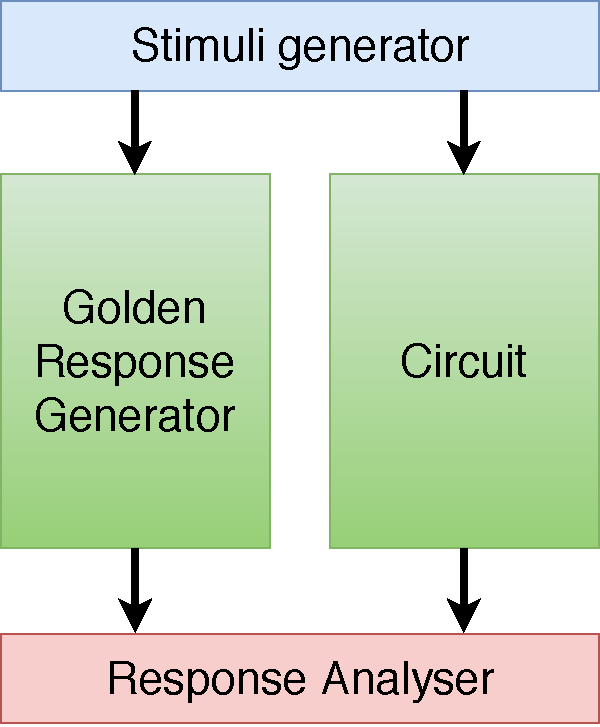
\includegraphics[width=0.25\textwidth]{Figures/Testbench.pdf}
	\caption{Test bench diagram.}
	\label{fig:tb}
\end{figure}

The results provided by the testbench might depend on the chosen simulator. This
happens because simulators work in different ways: while some focus on obtaining
the most complete results (including simulation timings), sacrificing the speed
of the simulations, others do the opposite. In this perspective, the simulators
can be divided into two main categories~\cite{tan:vhstas,palnitkar:verilog}:
event-driven or cycle-accurate.

As it will be seen in this Section, from all the simulators studied the one that
is the most suitable to reach the objectives defined for the new simulation
environment of the RV32-Versat architecture is Verilator: it is faster than the
more traditional event-driven simulators, it is inexpensive and allows the use
of C++ and SystemC to write the testbenches, therefore simplifying the creation
of a software and hardware co-simulation environment. Also, changes in the
hardware architecture will not require changes in the simulator.

\subsection{Event-Driven Simulators}
\label{section:event}

The first category of simulators are the event-driven
ones~\cite{tan:vhstas,gunes:survey,palnitkar:verilog}. Most of the commercially available 
simulators belong to this category, and they work by taking events sequentially, 
propagating them through the circuit until it reaches a steady state.

The events are generated each time that a circuit input is changed, being stored
in a queue, ordered chronologically to allow the correct execution of the
events. When an event is evaluated, only the circuit nodes that have their input
changed by that event are evaluated. After evaluation, the event is removed from
the queue, with new events that result from the output changes being added to
the queue. This means that the same element might be evaluated multiple times
during the same time step due to the feedback from some signals.

It is important to mention that during the simulation process there is a timer
that is used to keep track of the events timings. This leads to one of the main
advantages of event-driven simulation, which is the accurate simulation results,
with detailed timing information, allowing the identification of timing problems
in the tested circuit.

Despite this important advantage, this type of simulation also brings some
disadvantages, mainly related with its speed. Due to their complex algorithms
used for event scheduling and timing evaluation, event-driven simulators are
slow. While for relatively small circuits this might not be a significant
problem, for large circuits this is an important disadvantage, because their
increased complexity will increase significantly the simulation duration.

Event-driven simulators are the most common type of simulators, including
simulators like the Cadence NCSim~\cite{cadence:ncsim}, the Synopsys
VCS~\cite{synopsys:vcs}, the Mentor Graphics ModelSim~\cite{mentor:modelsim} or
the free of charge open source Icarus Verilog~\cite{icarus:verilog}. Usually,
they run on a general purpose computer, being divided into three categories,
according to their algorithms: compiled-code, interpreter and gate level.

An interpreter software simulator reads the \ac{HDL} code to simulate and interprets
it, translating the original code to a set of instructions accepted by the
simulator program. This translation process occurs during runtime and implies
the creation of data structures to store the data taken from the \ac{HDL} file, that
will be used afterwards to create the simulation. These simulators are somewhat
inefficient, due to the resultant overhead of the code translation. This
typically results in the execution of a considerable number of instructions per
element evaluation, of which only a few perform logic model
evaluation~\cite{lewis:compiled}. Icarus Verilog belongs to this category: it uses a 
compiler called iverilog to compile the \ac{HDL} circuit description into the vvp 
assembly format, accepted by the simulator. After this the vvp file generated is run by 
the simulator to execute the simulation.

On the other hand, a compiled-code simulator works by transforming the \ac{HDL}
circuit description, including its testbench, into an equivalent C code (or some
similar programming language). The generated code is then compiled by a generic
complier (like gcc, for example), resulting in an executable file, that will the
be executed to run the simulation. This type of simulators are more efficient
than the interpreter ones, since they eliminate the overhead of traversing the
network data structures~\cite{lewis:compiled}. The most used simulators, like
Cadence NCSim or Synopsys VCS, belong to this category of simulators.

Although the gate level simulators are either of the interpreted or
compiled-code type, they differ from the simulators referred in those
categories~\cite{tan:vhstas}. This happens because, while those simulators have
full Verilog compliance (supporting also gate level simulations), the gate level
simulators just support a small subset of Verilog.

\ac{RTL} simulation is the most used method for circuit verification due to its
reasonable accuracy~\cite{sousa:reconfigurable}. However, in the last few years
there has been a rising trend in the industry to run gate level
simulations~\cite{khandelwal:gatelevel}. This happens mainly due to the more
complex timing checks required by modern process nodes. As a result, despite
gate level simulation being more time consuming than \ac{RTL} simulation, it greatly
improves the verification results.

\subsection{Cycle-Accurate Simulators}
\label{section:cycle}

Cycle-Accurate simulators are another important category of HDL
simulators. Instead of taking events sequentially, propagating them through the
circuit until it reaches a steady state, like the event-driven simulators, this
type of simulators evaluate each logic element of the circuit in a clock
cycle. They do this evaluation for each clock cycle, without taking into
consideration the propagation times and delays within the
cycle~\cite{khandelwal:gatelevel}.

As a result, these simulators are considerably faster than the event-driven
ones. However, they provide incomplete information about the circuit, since they
do not evaluate the delays and propagation times when evaluating each clock
cycle. So, if a circuit has timing problems, a cycle-accurate simulator will not
be able to notice them, making necessary the use of an event-driven simulator at
some stage to evaluate the existence of timing problems. All these
characteristics make the cycle-accurate simulators best suited for large circuit
simulation, like CPUs, when simulation speed is an important factor.

Most cycle-accurate simulators use a 2-state model (0 or 1) to calculate the
values of the signals through the circuit. A typical event-driven simulator uses
a more complex model, with more states (adding states like undefined, unknown or
high-impedance)~\cite{bennett:verilator}. This means that cycle-accurate
simulators have to make assumptions when the signals may have a value different
from 0 or 1 (for example, a signal that was uninitialized). While this speeds up
the simulation process, it also might be prone to produce wrong results.

From all the cycle-accurate simulators available, the most used one is probably
Verilator. Verilator is an open source simulator that compiles synthesizable
Verilog RTL, generating cycle accurate C++ and SystemC models. For each circuit, Verilator
compiles a different model. These models are
then linked to a testbench, being executed in order to generate the
simulation. Verilator does not only translate Verilog code to C++ or
SystemC. Instead, it compiles the code into a much faster optimized and
thread-partitioned model, which is in turn wrapped inside a C++/SystemC
module~\cite{veripool:verilator}, that can be used afterwards in a software and hardware 
co-simulation environment.

\subsection{Hardware-based Simulators}
\label{subsection:hardware}

As the name indicates, hardware-based simulators are a type of simulators that
rely on configurable hardware to do the digital circuit verification. When
compared with the software-based simulators presented previously (event-driven and 
cycle-accurate), they have the advantage of being a
few orders of magnitude faster~\cite{tan:vhstas}. However they also have some
disadvantages: the hardware can be costly and it requires long compilation times, which 
makes them needless for smaller designs. These simulators also require proprietary 
hardware platforms to perform the desired simulations, with the hardware setup depending
on the platforms used, being different on each platform. As a result, these type
of simulators have a steep learning curve.

In this simulation type, the Verilog design is mapped onto a reconfigurable
piece of hardware with the same logical behaviour as the netlist.  The simulation
is divided between the software simulator, which simulates all the Verilog code
that is not synthesizable, and the hardware accelerator, which simulates
everything that is synthesizable~\cite{khandelwal:gatelevel}. The design is then
run on the hardware, producing the simulation results. The results, like in a
Software-based simulator, must be checked in order to assess if the circuit is
working properly.

There are two variants of Hardware-based simulators: \ac{FPGA}-based or
emulator-based. Emulator-based simulators offer the possibility of testing the software 
before having it implemented on chip, as the software application can run exactly as it
would on the real chip in a real system.

\subsection{Performance Comparison}
\label{section:performance}

In Figure~\ref{fig:performance} a chart comparing the performance of the most
popular Verilog software-based simulators available in the 
market~\cite{verilator:benchmarks} is shown. To run these benchmarks, a slightly modified 
model of the Motorolla M68K processor is used as the design under test. All the 
simulators shown were run on a general purpose computer with an 2.2GHz AMD Phenom 9500 
processor, 667MHz DDR2 Memory and running the SuSE 11.1 operating system. The benchmark
measures the number of clock cycles that a simulator can run in a fixed amount
of time, so a higher result means that the simulator has a better performance.

From the analysis of the benchmark results, it can be concluded that Verilator
is considerably faster than the other tested simulators, both in 32 and 64 bits
versions. Cadence NCSim is almost 2 times slower than Verilator, while Synopsis
VCS is 3.5 times slower. Icarus Verilog is the slowest simulator tested, being
almost 80 times slower than Verilator. This result was expected if we take into
account that Verilator is a cycle-accurate simulator, while the other simulators
are event-driven. Recall that event-driven simulators have lower performance
despite offering more detailed simulations. Among the event-driven simulators,
Icarus Verilog is the slowest since it is of the interpreter type while the
others are of the compiled-code type. Therefore, Icarus has to deal with the
overhead of code translation, as explained before.

\begin{figure}[!htb]
	\centering
	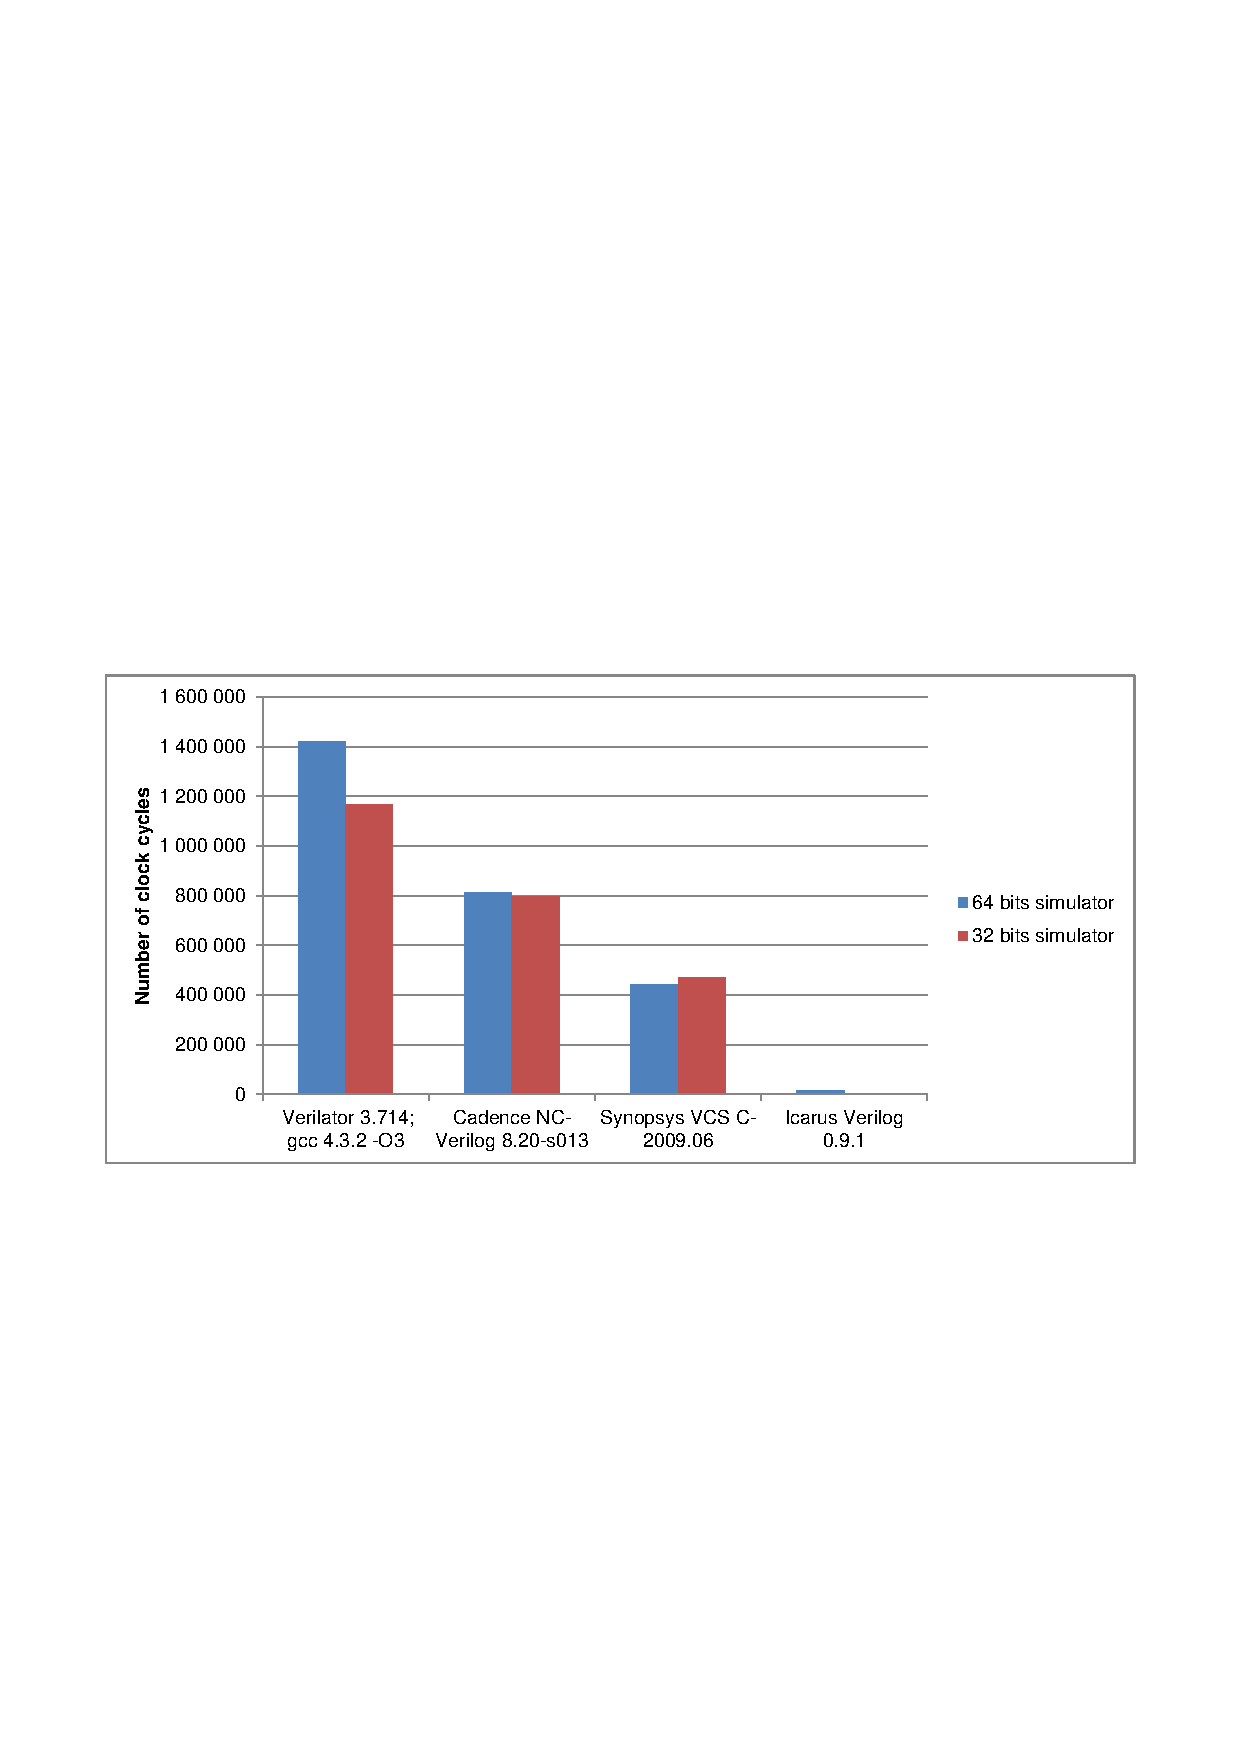
\includegraphics[trim=0 280 0 310 , clip, 
	width=0.5\textwidth]{Figures/Performance.pdf}
	\caption{Benchmark results for different HDL simulators~\cite{verilator:benchmarks}.}
	\label{fig:performance}
\end{figure}

The benchmark results shown should only work as reference, given their
limitations: the versions of the simulators used are already outdated, the same
happening with the hardware and operating systems used in the general purpose
computers. Also, this benchmark only evaluates the performance in one model
(Motorolla M68K processor), instead of using multiple models in order to provide
more accurate results.


\subsection{CGRA Simulation}
\label{section:CGRA}

Simulating CGRAs with event-driven simulators will result in
lengthy simulation times, since the reconfigurable
interconnects between the functional units allow building a multitude of
different datapaths at run-time. Consequently, finding a valid alternative to simulate
\ac{CGRA}s (in this particular case, the Versat architecture) could save an
important amount of time and money during the development of applications for
this type of architectures.

Using cycle-accurate simulators could be a good alternative to speed up
\ac{CGRA} simulations. As seen in the previous Section, the use of a
cycle-accurate simulator like Verilator could considerably cut the simulation
time, reducing it, at least, by a factor of 2 (see
Fig~\ref{fig:performance}). It also has the advantage of having no additional
cost, since Verilator is open source. However, the \ac{CGRA} (or any other
circuit) should not be tested exclusively with a cycle-accurate simulator, since
their results do not take into account the propagation delays inside the
\ac{CGRA}, and also make some simplifications regarding the signal states. This
is specially true if the \ac{CGRA} is in constant development.

Another alternative is doing simulations at a high-level, instead of doing them
at the \ac{RTL} level. High-level simulation techniques have been applied in
different types of circuits, like processors, with good results. However, for
\ac{CGRA} there is an additional difficulty compared to regular processors for
this type of simulations because of the reconfiguration process. Two examples of
approaches to high-level simulation were studied: one that proposes a
cycle-accurate simulator~\cite{chen:CGRA}, and another one that proposes a
framework for high-level simulation of \ac{CGRA}s~\cite{pasha:CGRA}. However,
both approaches have a problem: they are specifically tailored for an
architecture, so each time there is a significant change in the architecture,
the simulators will also need to be changed. With Verilator, for example, that
does not happen.

%%%%%%%%%%%%%%%%%%%%%%%%%%%%%%%%%%%%%%%%%%%%%%%%%%%%%%%%%%%%%%%%%%%%%%%%%%%%%%%%%%%%%%%%%%

\section{Simulating the RV32-Versat architecture using event-driven simulators}
\label{chapter:sim_event}

In this section is detailed the simulation environment for the RV32-Versat architecture 
using commercially available event-driven simulators, more specifically the Cadence NCsim 
and Synopsys VCS simulators. As explained in the previous section, both work by taking 
events sequentially, propagating them through the circuit until it reaches a steady 
state~\cite{tan:vhstas,gunes:survey,palnitkar:verilog}, producing accurate simulation 
results with detailed timing information, at the cost of the simulation speed.

\lstset{language=verilog}
\lstset{basicstyle=\scriptsize}
\begin{figure}[!htb]
	\begin{minipage}{\linewidth}
		\begin{lstlisting}[frame=single]
		`timescale 1 ns / 1 ps
		
		module system_tb;
		reg clk = 1;
		always #5 clk = ~clk;
		
		reg resetn = 0;
		
		initial begin
		`ifdef VCD
		$dumpfile("system.vcd");
		$dumpvars();
		`endif
		repeat (100) @(posedge clk);
		resetn <= 1;
		end
		
		wire          led;
		wire          ser_tx;
		wire          trap;
		reg           databus_sel;
		reg           databus_rnw;
		reg [14:0]    databus_addr;
		reg [31:0]    databus_data_in;
		
		system uut (
		.clk             (clk        ),
		.resetn          (resetn     ),
		.led             (led        ),
		.databus_sel     (databus_sel),
		.databus_rnw     (databus_rnw),
		.databus_addr    (databus_addr),
		.databus_data_in (databus_data_in),
		.ser_tx          (ser_tx     ),
		.trap            (trap       )
		);
		
		initial begin
		databus_sel = 0;
		databus_rnw = 1;
		databus_addr = 0;
		databus_data_in = 0;
		end
		
		always @(posedge clk) begin
		if (resetn && trap) begin
		$finish;
		end
		end
		endmodule
		\end{lstlisting}
	\end{minipage}
	\caption{Example testbench in Verilog for RV32-Versat}
	\label{fig:tb_verilog}
\end{figure}
\lstset{basicstyle=\normalsize}

\subsection{Testbench}
\label{section:tb}

This type of simulators work with testbenches written in an \ac{HDL} such as
Verilog or VHDL. In Figure~\ref{fig:tb_verilog}, an example of a simple
testbench written in Verilog and used by NCSim and VCS is shown. This testbench
has RV32-Versat as the \ac{UUT} and uses a clock period of 10 ns, meaning that
the system is simulated at a frequency of 100 MHz. After 100 clock cycles with
the reset enabled ({\tt resetn=0}) the reset is disabled, and RV32-Versat starts
running. The data bus external ports are not used, since the memories are
initialized at compile time and no input hex file is loaded by the
testbench. The simulation finishes when the trap signal is activated (with {\tt
	resetn=0}), and if the flag VCD is passed when running the simulator a \ac{VCD}
file will be generated. The trap signal is activated when there is an invalid
memory access, which is useful for debug and for stopping the simulation, which
is caused by the user software that intentionally accesses the memory at a non
mapped location.

\subsection{Verilog VPI}
\label{section:vpi}

The downside of using an HDL testbench with the event-driven simulators is their
limited support for software and hardware co-simulation. One way to overcome
this problem is to use the \ac{VPI}~\cite{vpi}, a C-programming interface for
Verilog that consists in a set of access and utility routines that are called
from standard C programming language functions. These routines interact with the
instantiated simulation objects contained in the Verilog design.

\lstset{language=C}
\lstset{basicstyle=\scriptsize}
\begin{figure}[!htb]
\begin{minipage}{\linewidth}
\begin{lstlisting}[frame=single]
#include "vpi_user.h"
			
void example() {
	vpi_printf("Example function\n");
	return;
}
\end{lstlisting}
\end{minipage}
\caption{Example C code for the VPI}
\label{fig:vpi_c}
\end{figure}
\lstset{basicstyle=\normalsize}

To better explain how the~\ac{VPI} works there is a simple example of a C
function in Figure~\ref{fig:vpi_c}, called {\tt example.c} that prints text in
the terminal, using the {\tt printf} function from the \ac{VPI}. This function
now needs to be associated with a system task. For this, a special data
structure needs to be created, of the type {\tt vpi\_systf\_data}. The code for
the creation and registration of the system task can be seen in
Figure~\ref{fig:vpi_routine}. After this stage, the system task must be called
in the Verilog testbench of the circuit to simulate. This can be done either in
{\tt initial} blocks or in {\tt always} blocks. In Figure~\ref{fig:vpi_verilog}
an example using an {\tt initial} block is shown. The last thing to do is
linking the task with the simulator. This is usually made in the terminal when
calling the simulator.

\lstset{language=C}
\lstset{basicstyle=\scriptsize}
\begin{figure}[!htb]
\begin{minipage}{\linewidth}
\begin{lstlisting}[frame=single]
#include "example.c"

void hello_register()
{
	s_vpi_systf_data tf_data;
	
	tf_data.type      = vpiSysTask;
	tf_data.tfname    = "$hello";
	tf_data.calltf    = hello_calltf;
	tf_data.compiletf = hello_compiletf;
	of the task
	
	vpi_register_systf(&tf_data);
}

//Register the new task
void (*vlog_startup_routines[ ]) () = {
hello_register,
0
;}
			
\end{lstlisting}
\end{minipage}
\caption{VPI task creation and registration}
\label{fig:vpi_routine}
\end{figure}

\lstset{language=Verilog}
\begin{figure}[!htb]
\begin{minipage}{\linewidth}
\begin{lstlisting}[frame=single]
module example ();

	initial begin
	$hello;
	#10 $finish;
	end

endmodule
\end{lstlisting}
\end{minipage}
\caption{Verilog code to invoke the task}
\label{fig:vpi_verilog}
\end{figure}
\lstset{basicstyle=\normalsize}

As it can be seen, although it is possible to do software and hardware
co-simulation using Verilog testbenches, the process is not direct, making it a
disadvantage in simulation environments based on event-driven simulators. If the
low performance of this type of simulators is also taken into account (as it can
be seen in the benchmarks in Section~\ref{section:benchmark}), it can be
concluded that a simulation environment based on event-driven simulators does
not reach the objectives pretended: it is not fast, the simulators licences are
expensive and it does not provide a straightforward way of integrating hardware
and software co-simulation. Therefore, an alternative is necessary.  There is
another event-driven simulator (Icarus Verilog) that could solve the cost
problems, since it is free, but this simulator does not support the {\tt
	generate} loops used in the RV32-Versat Verilog code and has a very low
performance, as seen in Section~\ref{section:performance}.

%%%%%%%%%%%%%%%%%%%%%%%%%%%%%%%%%%%%%%%%%%%%%%%%%%%%%%%%%%%%%%%%%%%%%%%%%%%%%%%%%%%%%%%%%%

\section{Simulating the RV32-Versat architecture using the new Verilator environment}
\label{chapter:sim_verilator}

In this section is detailed the new simulation environment for the RV32-Versat 
architecture using Verilator. It was designed to overcome the disadvantages typical of 
the simulation environments based on the more traditional event-driven simulators, like 
the Cadence NCsim and the Synopsys VCS, as detailed in the previous sections: slow 
simulations, expensive licences and complicated integration of hardware and software 
co-simulation, many times leading to the use of ad hoc solutions.

\subsection{Working principle}
\label{section:working_principle}

The simulation environment created for RV32-Versat is based in a set of GNU
Makefiles~\cite{stallman:makefile}. In order to run the simulation environment
the user must go to the root of the RV32-Versat repository and type the command
{\tt make simulator\_name TEST=test\_name}, where the {\tt simulator\_name} is
the name of the desired simulator (Verilator) and {\tt test\_name} is the name
of the folder of the test (driving software program) that must be placed inside
of the folder {\tt tests/test\_name}. The test is compiled, the system memories
are initialized with the program code and data and the system is simulated, following the 
flow shown in Figure~\ref{fig:sim_flow}. This flow will be followed for any program that 
is created and simulated for this architecture.

\begin{figure}[!htb]
	\centering
	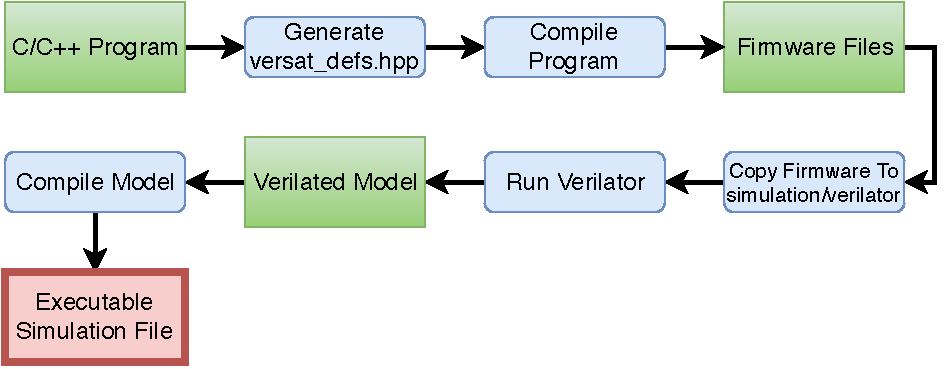
\includegraphics[width=0.48\textwidth]{Figures/Sim_flow.pdf}
	\caption{Simulation flow of the Verilator environment.}
	\label{fig:sim_flow}
\end{figure}

After the {\tt make} command is executed, the Makefile will call another
Makefile placed inside the folder {\tt simulation/verilator} that will then call
another Makefile placed inside the folder {\tt tests/test\_name}. This Makefile
generates the firmware hex files containing the RISC-V program and, if necessary, the 
data to be load into the Versat memories via the testbench, by generating the {\tt 
	versat\_defs.hpp} file and compiling the program using the RISC-V toolchain.

The generated firmware files will then be copied into the {\tt simulation/verilator} 
folder where the respective Makefile was called. The next step is to call
Verilator to generate the Verilated model, a C++/System C model obtained from the
synthesizable Verilog files. This model is then linked to the testbench and compiled 
using GNU g++. The resulting executable simulation file will be run and perform 
the actual simulation.

An additional option was added that allows the simulation to be run in machines
that do not have the RISC-V toolchain~\cite{gnu:riscv} installed. This option
compiles the program via SSH in a remote machine where the toolchain is properly
installed. With this option, the user does not need to install the toolchain in
the computer where the simulator is installed, since installing the RISC-V toolchain can 
be a lengthy and complicated process. This option can be activated by adding the flag 
{\tt TOOLCHAIN=FALSE} in the make command.

\subsection{The Verilator testbench}
\label{tb_verilator}

The Verilator testbench is considerably different from a typical HDL testbench,
mainly because it is written in C++, SystemC or a combination of both. The use
of these two languages instead of Verilog allows for much greater flexibility by
seamlessly emulating the software of a host system that stimulates the simulated
system. The testbench shown in Figure~\ref{fig:tb_cpp}, written in C++, works
essentially in the same way as the one shown in the previous Section
(Figure~\ref{fig:tb_verilog}): it loads the hex files to the Versat memories via
the data bus and then runs the program. The simulation finishes when the trap
signal in the PicoRV32 processor is activated, together with an indication that
the program has finished. Optionally, the simulation can output an hex file with
the contents of the Versat memories using the data bus external ports.

The C++ header file created by Verilator from the Verilog model (the Verilated
model) must be included in the C++ testbench. After this, the {\tt
	sc\_time\_stamp} function is invoked, so that the simulator knows the current
time. The simulation setup is done in the {\tt main} function: the runtime
arguments are analysed ( {\tt commandArgs}), the computation of the traced
signals is enabled ( {\tt traceEverOn}), the module to be simulated is declared
( {\tt Vsystem*top}), along with the Verilated VCD model ( {\tt VerilatedVcdC*
	tfp}) and the number of hierarchy levels to be traced are defined ( {\tt
	top->trace (tfp, 99)}). As with the Verilog testbench example, in this example
the data bus external ports are switched off in order to keep the example
simple.

The clock of the circuit is toggled inside the while cycle. For each time that
this cycle executed, the clock signal will be negated, the simulation time will
be checked (to verify if the reset has been disabled), the circuit will be
evaluated ({\tt top->eval()}), the signals will be written to the VCD file ({\tt
	tfp->dump(t)}) and the clock signal time will incremented by 5 ns in each half
period, resulting in a frequency of 100 MHz.The testbench will be executed until
the ( {\tt Verilated::gotFinish}) condition is true. This will happen when the
trap signal is activated and the reset disabled (resetn=1), making the program
leave the while cycle. This will finish the simulation and exit the testbench

\lstset{language=C++}
\lstset{basicstyle=\scriptsize}
\begin{figure}[!htb]
\begin{minipage}{\linewidth}
\begin{lstlisting}[frame=single]
#include "Vsystem.h"
#include "verilated.h"
#include "verilated_vcd_c.h"

vluint64_t main_time = 0; 
double sc_time_stamp () {
	return main_time;
}

int main(int argc, char **argv, char **env)
{
	Verilated::commandArgs(argc, argv);
	Verilated::traceEverOn(true);
	Vsystem* top = new Vsystem;
	VerilatedVcdC* tfp = new VerilatedVcdC;
	top->trace (tfp, 99);
	tfp->open ("waves.vcd");
	
	top->clk = 0;
	top->databus_sel = 0;
	top->databus_rnw = 1;
	top->databus_addr = 0;
	top->databus_data_in = 1;
	
	int t = 0;
	
	while (!Verilated::gotFinish()) {
		if (t > 200)
			top->resetn = 1;
		top->clk = !top->clk; //Toggle clock
		top->eval();          //Evaluate the model
		tfp->dump (t);        //Write to VCD file
		t += 5;               //Increment clock
		if (top->resetn && top->trap == 1)
			Verilated::gotFinish(true);
	}

	tfp->close(); //Close the VCD
	top->final(); //Finish the simulation
	delete top;
	exit(0);
}
\end{lstlisting}
\end{minipage}

	\caption{Example testbench in C++ for RV32-Versat}
	\label{fig:tb_cpp}
\end{figure}
\lstset{basicstyle=\normalsize}

Since the testbench is written in C++/SystemC, it is easy to do software and
hardware co-simulation, given that the host application can be directly embedded
in the testbench. This is a major improvement over other simulation environments
using Verilog testbenches. This is not the only advantage of this new
environment: the simulations using Verilator are considerably faster, as it can
be see in the benchmark presented in the Section~\ref{section:benchmark},
performed for the \ac{CNN} application presented in
Section~\ref{section:application}. Also, since Verilator is a completely free
open-source project, no licence fees are due. This advantages suit perfectly the 
objectives defined for the new simulation environment.
The major disadvantage of this new simulation environment is its lower
precision when compared with environments using event-driven simulators. This
happens because Verilator does not provide timing information, since it does not
take into account propagation times and because Verilator uses a 2-state model,
assuming that all the signals in a circuit have a value that can either be 0 or
1.  However, this disadvantage is many times irrelevant in the context of the
RV32-Versat architecture, since this architecture has already been extensively
tested in \ac{FPGA}s and with other simulators.

%%%%%%%%%%%%%%%%%%%%%%%%%%%%%%%%%%%%%%%%%%%%%%%%%%%%%%%%%%%%%%%%%%%%%%%%%%%%%%%%%%%%%%%%%%

\section{Results}
\label{chapter:results}

In this section the experimental results for the simulation environment developed for 
the RV32-Versat architecture are presented and discussed. In 
Section~\ref{section:benchmark} a comparison of the performance of the different 
simulators (Candece NCsim, Synopsys VCS and Verilator) is made, using the \ac{CNN} 
application developed during this paper.

\subsection{Simulator Performance Benchmarking}
\label{section:benchmark}

In order to test the performance of each one of the simulators discussed during this 
paper a benchmark was made. This benchmark consists in simulating the \ac{CNN} 
application (presented in~\ref{section:application}) running in the RV32-Versat 
architecture.

The benchmark consists of two tests: (1) using the simulators debug mode, which
enables internal assertions and debugging messages and generation of a \ac{VCD}
waveform file (debug+\ac{VCD} mode); (2) running the simulators without debug and
waveform file generation, and setting the -O3 {\tt g++} compiler flag when
compiling the Verilator model, which reduces the simulation time at the cost of
a slightly higher compile time (normal mode).

All this tests were executed in a 64 bit machine, with an Intel i5-4430 processor and 8 
GB of memory, running Ubuntu 16.04.3 LTS. The versions of the simulators used were the 
following: Verilator 4.014 (released in May 2019), Synopsys VCS 2017.03 (released in 
March 2017) and Cadence NCSim 13.10 (released in 2013). While
Verilator was at the most recent stable version available, for the other
simulators the versions used corresponded to the available software licences
made available by the Europractice service.

All the simulators were run in 64-bit mode using a single thread.The experimental results 
are presented graphically in Figures~\ref{fig:benchmark} and~\ref{fig:benchmark_vcd}.

\begin{figure}[!htb]
	\centering
	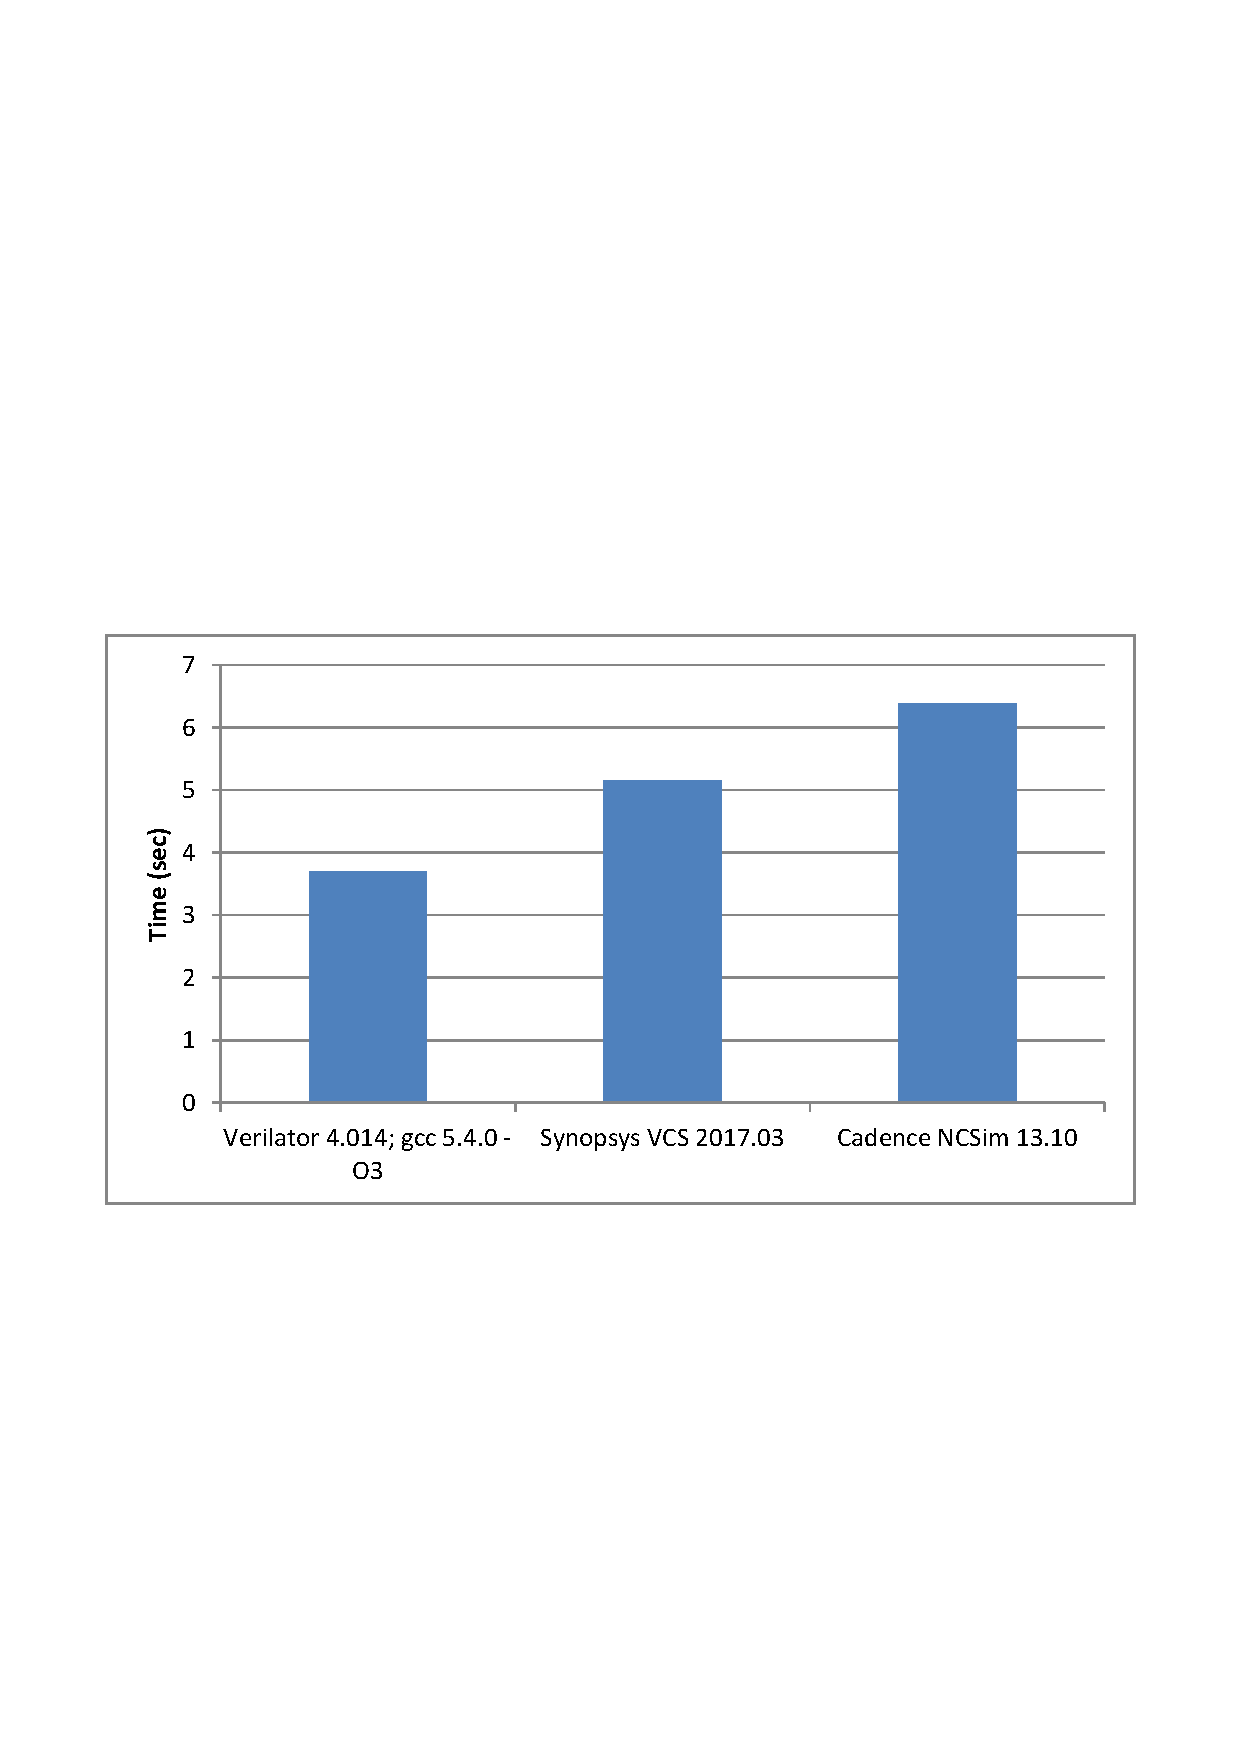
\includegraphics[trim=0 250 0 290 , clip, width=0.5\textwidth]{Figures/benchmark.pdf}
	\caption{Benchmark results for RV32-Versat running the convolutional neural network.}
	\label{fig:benchmark}
\end{figure}

\begin{figure}[!htb]
	\centering
	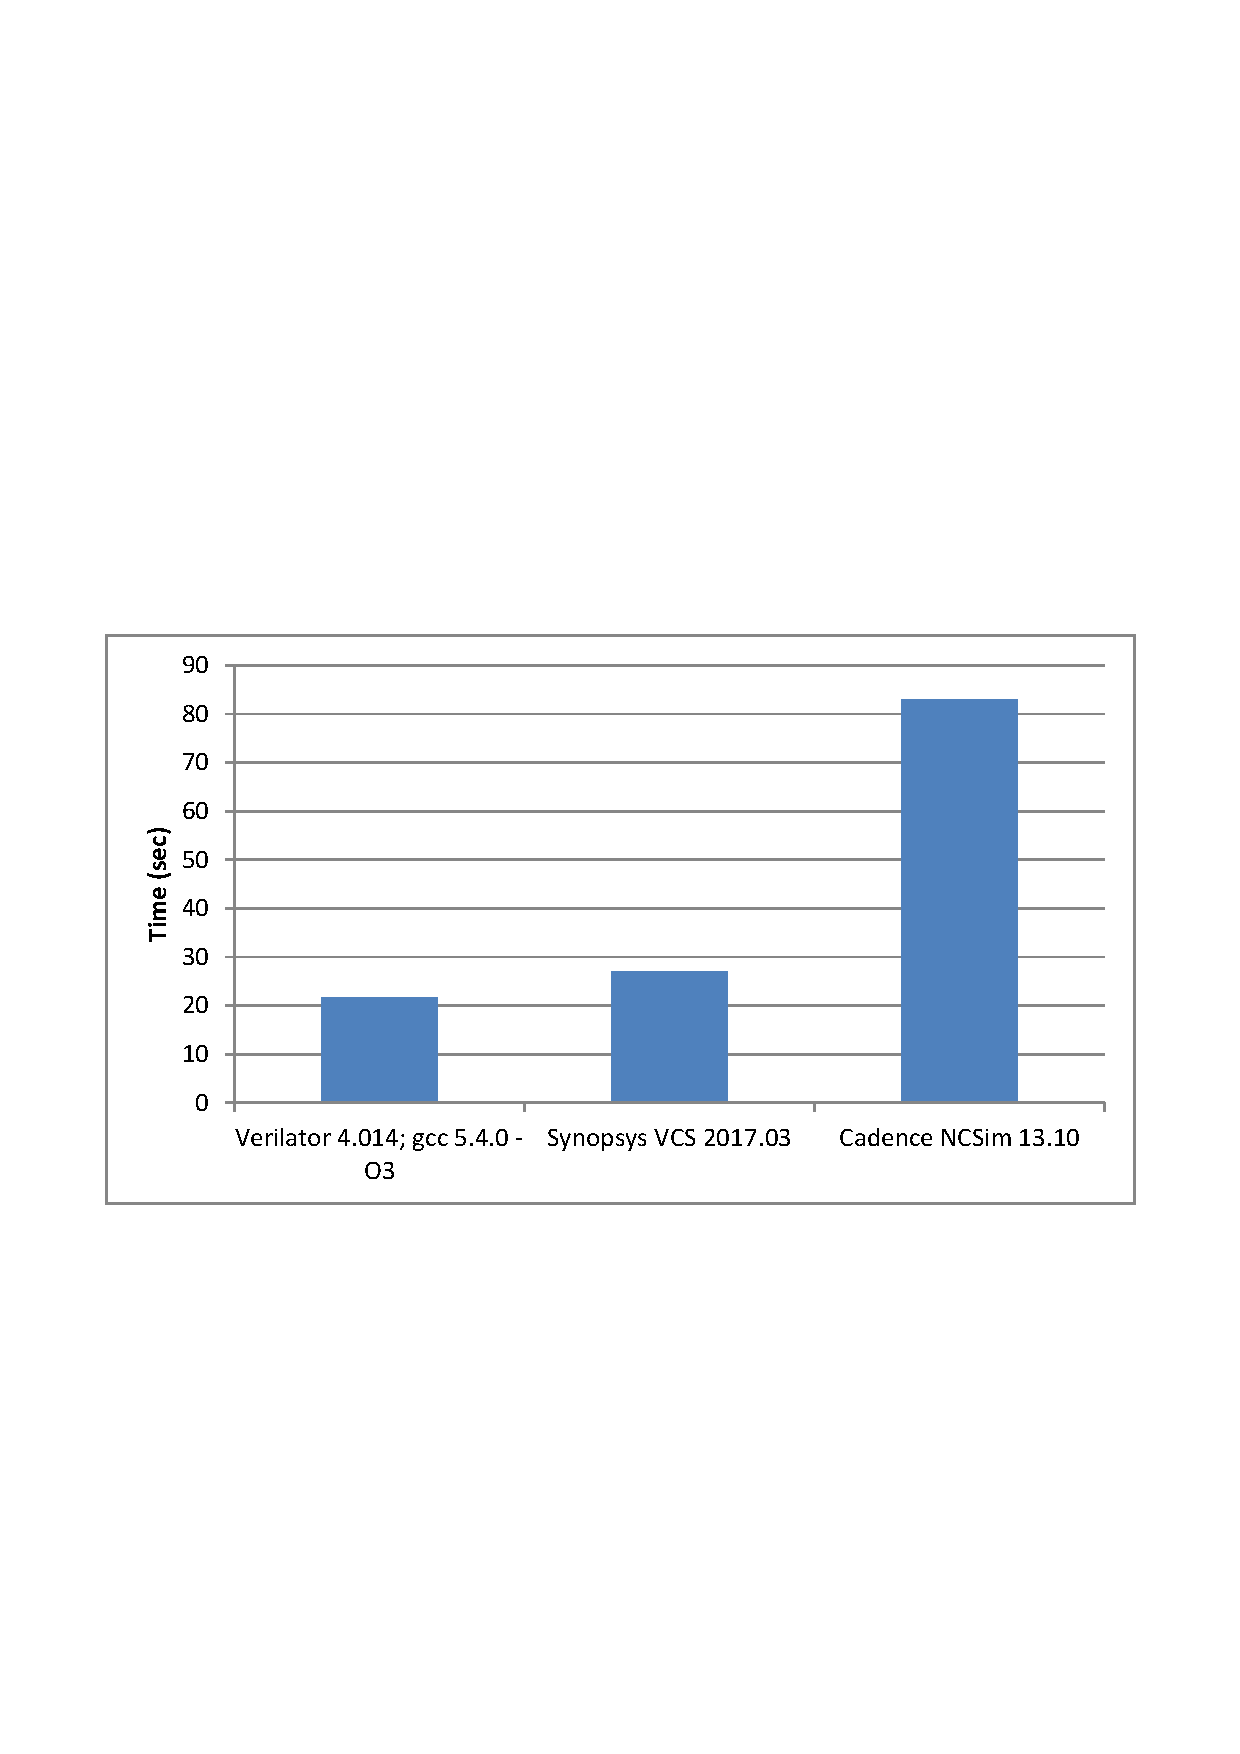
\includegraphics[trim=0 250 0 290 , clip, 
	width=0.5\textwidth]{Figures/benchmark_vcd.pdf}
	\caption{Benchmark results for RV32-Versat running the convolutional neural network. 
		Debug mode and
		vcd generation enabled.}
	\label{fig:benchmark_vcd}
\end{figure}

As expected, the simulation times are longer in the debug+\ac{VCD} mode, since more 
internal assertions are enabled and a considerable amounit of data is written to the 
computer disk. This was probably the main reason for the low performance of
NCsim, since it produced a \ac{VCD} file considerably larger than the other
simulators.

It can be seen that in both tests Verilator is the fastest simulator. This was
expected since Verilator is a cycle-accurate simulator whereas the other two are
event-driven simulators. Event-driven simulators are typically slower since the
algorithms used are more complex than the ones used in cycle-accurate
simulators, as explained in more detail in Section~\ref{section:performance}. The
second fastest simulator was Synopsys VCS, which was 1.39 and 1.24 times slower
than Verilator, for the normal and debug+\ac{VCD} modes, respectively. Finally, the
slowest simulator was Cadence NCSim, 1.73 and 3.81 times slower than
Verilator for the normal and debug+\ac{VCD} modes, respectively. As said before,
event-driven simulators (like Cadence NCSim or Synopsys VCS) provide more
detailed results, being specially useful in the early stages of development or
to simulate individual modules. However, RV32-Versat is a complex system and
each one of its modules has already been vastly tested, so it makes sense to
save time (and money) by using Verilator, since there is a low risk of getting
wrong simulation results due to the simplifications implemented by Verilator.

Comparing the above results with the ones obtained
in~\cite{verilator:benchmarks} and shown in Section~\ref{section:performance},
some differences can be noticed. In spite of Verilator being the fastest
simulator in both results, in this work the difference is smaller. Also, while
in~\cite{verilator:benchmarks} NCSim is the second fastest simulator, here that
does not happen and VCS is faster than NCSim, especially when the debug mode and
\ac{VCD} generation are enabled.

These differences can be caused by multiple factors: the computers used to run
the simulations were different, and the same applies to the simulated models:
in~\cite{verilator:benchmarks} a Motorolla M68K processor derivative was used
whereas here the RV32-Versat system was used. The versions of the simulators
used were also different, and that might be a reason for NCSim being
so slow compared to VCS. In fact, the NCSim version is from 2013. This of course
does not invalidate the results for the present work but it is worth noticing for
the sake of rigour.

%%%%%%%%%%%%%%%%%%%%%%%%%%%%%%%%%%%%%%%%%%%%%%%%%%%%%%%%%%%%%%%%%%%%%%%%%%%%%%%%%%%%%%%%%%

\section{Conclusions}
\label{chapter:conclusions}

In this paper the simulation environment developed for the RV32-Versat architecture was 
presented. This simulation environment presents a considerable improvement over the 
typical simulation environments using event-driven simulators: it is faster, it is 
inexpensive, not requiring the acquisition of licences, and allows a direct 
implementation of software and hardware co-simulation, avoiding the use of the \ac{VPI} 
or inefficient ad hoc solutions.

This ambient was developed after a detailed study of the state of the art of 
\ac{CPU} and \ac{CGRA} simulators, that did not only include the event-driven and 
cycle-accurate simulators, but also included custom simulators specifically developed for 
CGRAs. This was done to ensure that the simulation environment would correspond to the 
defined objectives.

To test the new simulation environment an application using a \ac{CNN} was developed and 
its results were compared with the ones obtained with the RV32-Versat architecture 
implemented in an \ac{FPGA}. This way it was possible to ensure that the results obtained 
with the new simulation environment were correct.

% ----------------------------------------------------------------------
\subsection{Achievements}
\label{section:achievements}


The first achievement of this paper was the development of a faster simulation 
environment. As it was seen in the benchmark presented in 
Section~\ref{section:benchmark}, this simulation environment can be up to 3.81 times 
faster than a simulation environment using the traditional event-driven simulators. This 
can help to cut the time needed to develop and debug applications for the RV32-Versat.

Another important achievement is the reduction of the amount of money spent in licences. 
This happens because the new simulation environment uses Verilator, an open-source 
simulator, in contrast to the event-driven simulators that require expensive licences. 
This is particularly useful for small companies, allowing them to spend their limited 
resources in other areas.

The third achievement is the improved support for hardware and software 
co-simulation in this new simulation environment, dismissing the use of special 
interfaces (like the Verilog \ac{VPI}) or ad hoc solutions. With this new environment the 
testbench can be written in C++ or SystemC, therefore allowing a seamless integration of 
hardware and software co-simulation.

The last achievement was the development of a simulation environment that is independent 
from eventual changes in the RV32-Versat architecture. This means that if the 
architecture of RV32-Versat is changed, the simulation environment will keep working. 
This would not happen if a simulator developed for this specific architecture was used, 
instead of Verilator.

%\section*{Acknowledgment}

%The preferred spelling of the word ``acknowledgment'' in America is without 
%an ``e'' after the ``g''. Avoid the stilted expression ``one of us (R. B. 
%G.) thanks $\ldots$''. Instead, try ``R. B. G. thanks$\ldots$''. Put sponsor 
%acknowledgments in the unnumbered footnote on the first page.

\bibliographystyle{unsrt}
% argument is your BibTeX string definitions and bibliography database(s)
\bibliography{Thesis_bib_DB}

\end{document}
